\documentclass [hw,noanswers]{exam}

\newcommand\myroot{..}
\usepackage{\myroot/physics_summer}

\title{Problem Set \#1: Intro kinematics}
\author{\mobeardInstructorShort}
\date{\printdate{6/15/2021}}
\duedate{\printdate{6/23/2021}}

\begin{document}
\maketitle

Suggested reading is chapter 1 of \citet{kleppner2014introduction}.

\begin{questions}
\question Typical problems (from \citet{hecht2018schaums})
\begin{parts}
\part A toy train moves along a winding track at an average speed of \SI{0.25}{\meter\per\second}. How far will it travel in \SI{4.00}{\minute}?
\begin{solution}
$ \SI{0.25}{\meter\per\second} \times \SI{4}{\minute} \times \dfrac{\SI{60}{\second}}{\SI{1}{\minute}} = \SI{60}{\meter}$
\end{solution}
\part A student driving a car travels \SI{10.0}{\kilo\meter} in \SI{30.0}{\minute}. What was her average speed?
\begin{solution}
$\SI{10.0}{\kilo\meter} \times \SI{0.5}{\hour} = \SI{5}{\kilo\meter\per\hour}$
\end{solution}
\part A model plane flew \SI{100}{\meter} in \SI{25.0}{\second} followed by another \SI{240}{\meter} in an additional \SI{60.0}{\second}, whereupon it crashed into the ground. How far did it travel in total? How long was it in the air? What was its average speed?
\begin{solution}
Total distance is \SI{340}{\meter}. Total time is \SI{85}{\second}. Average speed is \SI{4}{\meter\per\second}. 
\end{solution}
\end{parts}

\question\label{q:2} Xuan the guide dog puppy is riding in a 2000 Ford Ranger. He records his position versus time as shown in \fref{fig:q2}. Develop an appropriate equation for Xuan's position $x(t)$, velocity $v(t)$ and acceleration $a(t)$; write the equations and graph all three. Discuss some issues you may have in estimating the velocity and acceleration. 
\begin{figure}[h]
\begin{center}
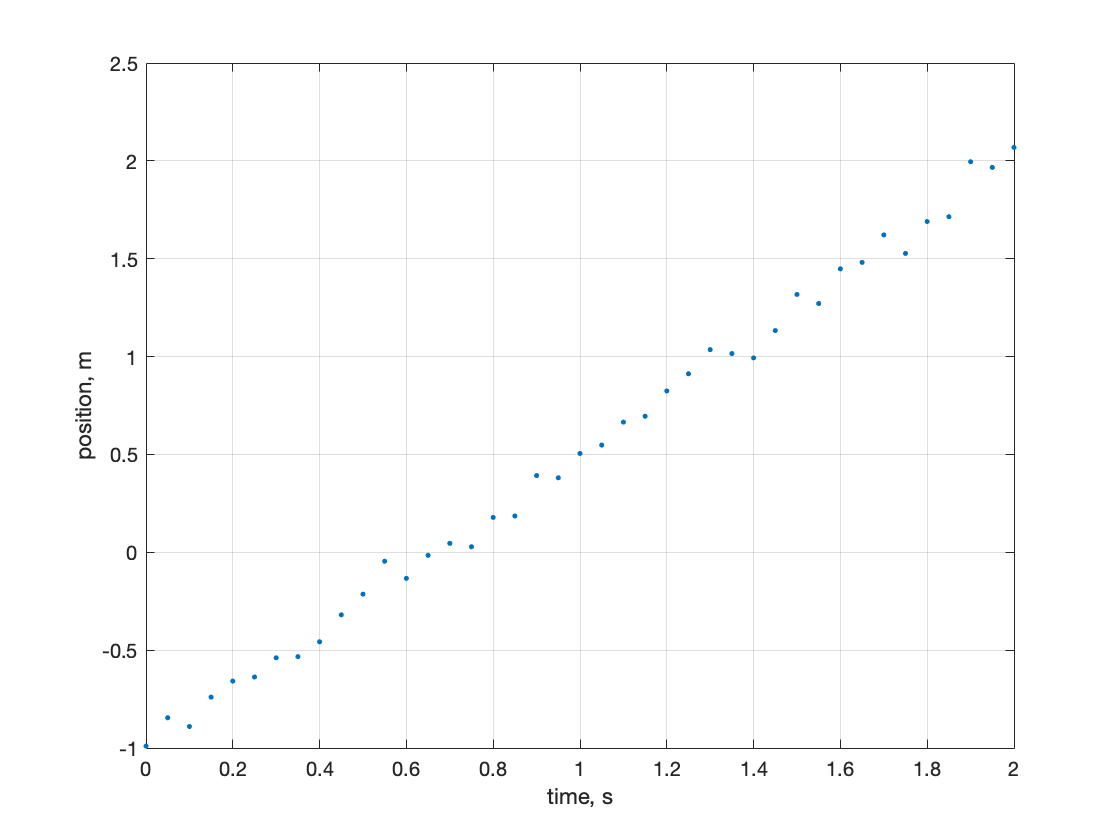
\includegraphics[width=0.75\columnwidth]{\myroot/figures/hw1p2.png}
\end{center}
\caption{Question~\ref{q:2}}
\label{fig:q2}
\end{figure}
\begin{solution}
Looking at the graph, it appears that $x(t)=1.5t-1$. Thus, velocity is $v(t)=1.5$, and $a(t)=0$. This is the constant velocity case we discussed. 

I might try to estimate $v$ by taking two adjacent measurements, subtracting them, and dividing by $\Delta t$. This data set has noise, however, which would throw off such estimates and would result in noisy estimates of $v$ and $a$. Our answer of $x(t)=1.5t-1$ depends on having a model and deciding it fits well enough to the data, and using perfect derivatives of that model to get velocity and acceleration... Differentiation injects noise each time we take a derivative, which could mask what we think the velocity and acceleration are without further filtering. 
\end{solution}

\clearpage
\question We developed expressions for $x(t)$, $v(t)$ and $a(t)$ for the case of constant velocity motion. Develop the same for the case of \textbf{constant acceleration}. 
\begin{parts}
\part What is $a(t)$ for \textbf{constant} acceleration? (not a trick question)
\begin{solution}
$a(t)=A\quad\text{(constant)}$
\end{solution}
\part\label{part:3b} What is $v(t)$? You may find this by finding the area under the $a(t)$ curve, or by using the integral. Recall that for $f(t)=at^b$, $\frac{df}{dt}=bat^{b-1}$, and $\int f dt = \frac{a}{b+1} t^{b+1}+C_1$, where $C_1$ is the constant of integration. 
\begin{solution}
Using the hint, $v(t)=At + C_1$. 
\end{solution}
\part What is $x(t)$? Again, you may find this by finding the area under the $v(t)$ curve, or by using the integral. Recall that for $f(t)=at^b$, $\frac{df}{dt}=bat^{b-1}$, and $\int f dt = \frac{a}{b+1} t^{b+1}+C_2$, where $C_2$ is the constant of integration. Try to do whichever one you didn't do during part~\ref{part:3b}. You will have a different constant of integration. 
\begin{solution}
Again using the hint, $x(t)=\frac{1}{2}A t^2 + C_1 t + C_2$. 
\end{solution}
\part Sketch all three functions $a(t)$, $v(t)$ and $x(t)$. How does your sketch change for different values of $C_1$ and $C_2$. What are the units of the constants $C_1$ and $C_2$, and what do they represent?. 
\begin{solution}
$C_1$ has units of \si{\meter\per\second} and represents the initial velocity. $C_2$ has units of \si{\meter} and represents the initial position. 
\end{solution}
\part Check your results by finding the slope (or derivatives) of $x(t)$ and $v(t)$. Try both. 
\begin{solution}
Taking derivatives gives $v(t)=\frac{dx}{dt}=At+C_1$, $a(t)=\frac{dv}{dt}=A$. Checks!
\end{solution}
\end{parts}

\question You move to LA and get a job at NASA JPL working on a small, zero G robot propelled with compressed air, able to move around inside the International Space Station. You are planning a set of commands to transmit to the robot for an upcoming flight test on a ``Vomit Comet'' C-9B microgravity simulator plane. 

\begin{parts}
\part The first test maneuver is to fly up \SI{1}{\meter} in \SI{1}{\second}, hover for \SI{1}{\second}, then return to the launch point in \SI{1}{\second}. Sketch the vertical position and velocity of the robot. You will need this to construct velocity commands to send to the robot, and to set failsafe limits on position in its autonomous flight controller.
\begin{solution}
Add sketch later. 
\end{solution}
\part During the actual test, a failure occurs in the propulsion system, resulting in the throttle valve being stuck open during the first part of the maneuver (heading upwards). With the failed valve, the force on the robot is \SI{10}{\newton} and its mass is \SI{1}{\kilo\gram}. Please plot the robot's position versus time. The far wall of the test chamber is \SI{10}{\meter} away; show when it hits the wall on your graph. Assume the robot is streamlined so that air resistance is small and neglect any change in mass from the expulsion of propellant.  
\begin{solution}
With the stuck valve, the robot experiences constant acceleration where $a=\dfrac{\SI{10}{\newton}}{\SI{1}{\kilo\gram}}=\SI{10}{\meter\per\second\squared}$. Thus, $a=10$, $v=10t$, and $x=5t^2$, assuming it starts at $x=0$ and $v=0$. 

Solving $x=5t^2$ for where $x=\SI{10}{\meter}$, the robot hits the wall at $t=\sqrt{2}=\SI{1.4}{\second}$. 
\end{solution}
\part To think about design changes in case of another similar failure, we need to know how long the robot has to respond, and how bad it is when it hits. Please compute the time to hitting the wall, and the speed when it hits. 
\begin{solution}
The time to hit the wall is $t=\SI{1.4}{\second}$ from above; this is the time the robot has to recognize the fault and try to correct. If it fails to correct, the speed at which it will hit the wall is $v=10\times\SI{1.4}{\second}=\SI{14}{\meter\per\second}$.  

We could then assess if this speed is fast enough to be a hazard; think of ways to restrict the thrust so as not to reach unacceptably high speeds or require very quick response times, or assess installation of multiple throttle valves to reduce the risk of a failure. 
\end{solution}
\end{parts}
\end{questions}

\bibliography{\myroot/physics9}
\end{document}
